\documentclass[tikz,border=12pt]{standalone}
\usepackage{tikz}
\usetikzlibrary{arrows.meta}

\definecolor{fairblue}{RGB}{33, 102, 172}
\definecolor{fairmidblue}{RGB}{103, 169, 207}
\definecolor{fairlight}{RGB}{247, 247, 247}
\definecolor{fairmidred}{RGB}{239, 138, 98}
\definecolor{fairred}{RGB}{178, 24, 43}
\definecolor{darkgray}{RGB}{60, 60, 60}
\definecolor{lightgrid}{RGB}{230, 230, 230}

\begin{document}
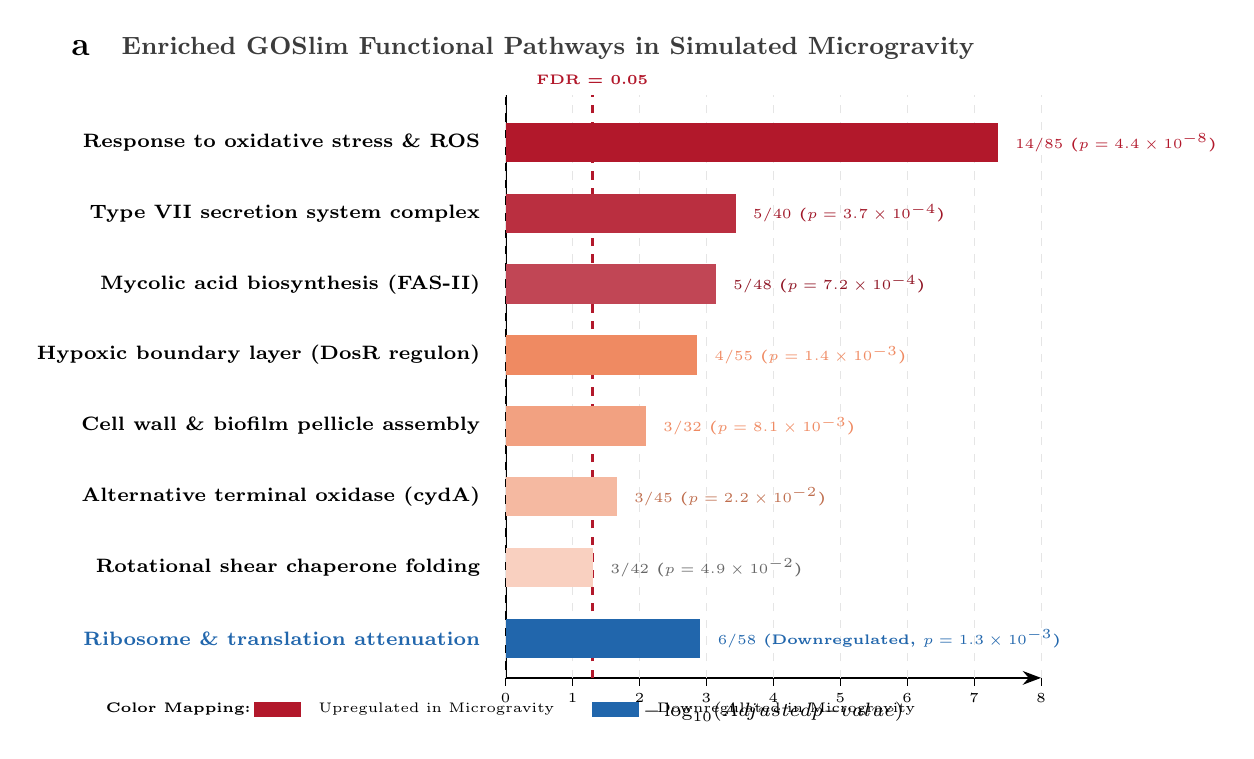
\begin{tikzpicture}[font=\sffamily, >=Stealth]
  % Title / Header
  \node[font=\large\bfseries] at (0, 8.8) {a};
  \node[anchor=west, font=\small\bfseries, text=darkgray] at (0.4, 8.8) {Enriched GOSlim Functional Pathways in Simulated Microgravity};

  % Horizontal Bar Plot Axes
  \draw[->, thick] (5.4, 0.8) -- (12.2, 0.8) node[midway, below=5pt, font=\scriptsize\bfseries] {$-\log_{10}(\text{Adjusted } p\text{-value})$};
  \draw[thick] (5.4, 0.8) -- (5.4, 8.2);

  % Axis Ticks
  \foreach \x/\lbl in {5.4/0, 6.25/1, 7.1/2, 7.95/3, 8.8/4, 9.65/5, 10.5/6, 11.35/7, 12.2/8} {
    \draw (\x, 0.7) -- (\x, 0.8) node[below=2pt, font=\tiny] {\lbl};
    \draw[dashed, draw=gray!20] (\x, 0.8) -- (\x, 8.2);
  }
  
  % Significance Threshold line at FDR = 0.05 (-log10 = 1.30)
  \draw[dashed, draw=fairred, line width=1pt] (6.5, 0.8) -- (6.5, 8.2) node[above, font=\tiny\bfseries, text=fairred] {FDR = 0.05};

  % Bars (Y positions: 7.6, 6.7, 5.8, 4.9, 4.0, 3.1, 2.2, 1.3)
  
  % 1. Response to oxidative stress & ROS (padj = 4.4e-8 -> mlog10 = 7.35) -> Deep Red
  \node[anchor=east, font=\scriptsize\bfseries] at (5.2, 7.6) {Response to oxidative stress \& ROS};
  \fill[fairred] (5.4, 7.35) rectangle (11.65, 7.85);
  \node[anchor=west, font=\tiny\bfseries, text=fairred] at (11.75, 7.6) {$14/85$ ($p=4.4\times 10^{-8}$)};

  % 2. Type VII secretion system complex (padj = 3.7e-4 -> mlog10 = 3.43) -> Red
  \node[anchor=east, font=\scriptsize\bfseries] at (5.2, 6.7) {Type VII secretion system complex};
  \fill[fairred!90!white] (5.4, 6.45) rectangle (8.32, 6.95);
  \node[anchor=west, font=\tiny\bfseries, text=fairred!90!black] at (8.42, 6.7) {$5/40$ ($p=3.7\times 10^{-4}$)};

  % 3. Mycolic acid biosynthesis (FAS-II) (padj = 7.2e-4 -> mlog10 = 3.14) -> Red
  \node[anchor=east, font=\scriptsize\bfseries] at (5.2, 5.8) {Mycolic acid biosynthesis (FAS-II)};
  \fill[fairred!80!white] (5.4, 5.55) rectangle (8.07, 6.05);
  \node[anchor=west, font=\tiny\bfseries, text=fairred!80!black] at (8.17, 5.8) {$5/48$ ($p=7.2\times 10^{-4}$)};

  % 4. Hypoxic boundary layer (DosR regulon) (padj = 1.39e-3 -> mlog10 = 2.86) -> Mid-Red
  \node[anchor=east, font=\scriptsize\bfseries] at (5.2, 4.9) {Hypoxic boundary layer (DosR regulon)};
  \fill[fairmidred] (5.4, 4.65) rectangle (7.83, 5.15);
  \node[anchor=west, font=\tiny\bfseries, text=fairmidred] at (7.93, 4.9) {$4/55$ ($p=1.4\times 10^{-3}$)};

  % 5. Cell wall & biofilm pellicle assembly (padj = 8.1e-3 -> mlog10 = 2.09) -> Mid-Red
  \node[anchor=east, font=\scriptsize\bfseries] at (5.2, 4.0) {Cell wall \& biofilm pellicle assembly};
  \fill[fairmidred!80!white] (5.4, 3.75) rectangle (7.18, 4.25);
  \node[anchor=west, font=\tiny\bfseries, text=fairmidred] at (7.28, 4.0) {$3/32$ ($p=8.1\times 10^{-3}$)};

  % 6. Alternative terminal oxidase (cydA) (padj = 2.17e-2 -> mlog10 = 1.66) -> Light Red
  \node[anchor=east, font=\scriptsize\bfseries] at (5.2, 3.1) {Alternative terminal oxidase (cydA)};
  \fill[fairmidred!60!white] (5.4, 2.85) rectangle (6.81, 3.35);
  \node[anchor=west, font=\tiny\bfseries, text=fairmidred!80!black] at (6.91, 3.1) {$3/45$ ($p=2.2\times 10^{-2}$)};

  % 7. Rotational shear chaperone folding (padj = 4.96e-2 -> mlog10 = 1.30) -> Light Red
  \node[anchor=east, font=\scriptsize\bfseries] at (5.2, 2.2) {Rotational shear chaperone folding};
  \fill[fairmidred!40!white] (5.4, 1.95) rectangle (6.51, 2.45);
  \node[anchor=west, font=\tiny\bfseries, text=gray!80!black] at (6.61, 2.2) {$3/42$ ($p=4.9\times 10^{-2}$)};

  % 8. Ribosome & translation attenuation (padj = 1.25e-3 -> mlog10 = 2.90) -> DEEP BLUE (Downregulated!)
  \node[anchor=east, font=\scriptsize\bfseries, text=fairblue] at (5.2, 1.3) {Ribosome \& translation attenuation};
  \fill[fairblue] (5.4, 1.05) rectangle (7.87, 1.55);
  \node[anchor=west, font=\tiny\bfseries, text=fairblue] at (7.97, 1.3) {$6/58$ (Downregulated, $p=1.3\times 10^{-3}$)};

  % Legend
  \node[font=\tiny\bfseries, anchor=west] at (0.2, 0.4) {Color Mapping:};
  \fill[fairred] (2.2, 0.3) rectangle (2.8, 0.5); \node[font=\tiny, anchor=west] at (2.9, 0.4) {Upregulated in Microgravity};
  \fill[fairblue] (6.5, 0.3) rectangle (7.1, 0.5); \node[font=\tiny, anchor=west] at (7.2, 0.4) {Downregulated in Microgravity};
\end{tikzpicture}
\end{document}
